%==================== chapter3_1.tex ====================

\clearpage
\thispagestyle{plain}

\begingroup
\fontsize{16pt}{19.2pt}\selectfont
\justifying
\XeTeXlinebreakskip=0pt plus 1pt minus 0.5pt
\setlength{\parindent}{1.5cm}
\setlength{\parskip}{0pt}

% ---------- หัวข้อใหญ่ (ชิดซ้าย, หนา 16pt) ----------

\section*{Use Case Diagram}
\addcontentsline{toc}{section}{Use Case Diagram}

% ---------- เนื้อหา (จัดกระจายแบบไทย, ย่อหน้าแรก 1.5 ซม.) ----------
\indent Use Case Diagram ที่เป็นการจำลองการทำงานของผู้เข้าประกวดผู้เชี่ยวชาญและฝ่าย
ประชาสัมพันธ์ซึ่งจะเห็นได้ว่าระบบนี้ประกอบไปด้วย 27 Use Case Diagram คือ

\vspace{\baselineskip}

\begin{figure}[h]
	\centering
	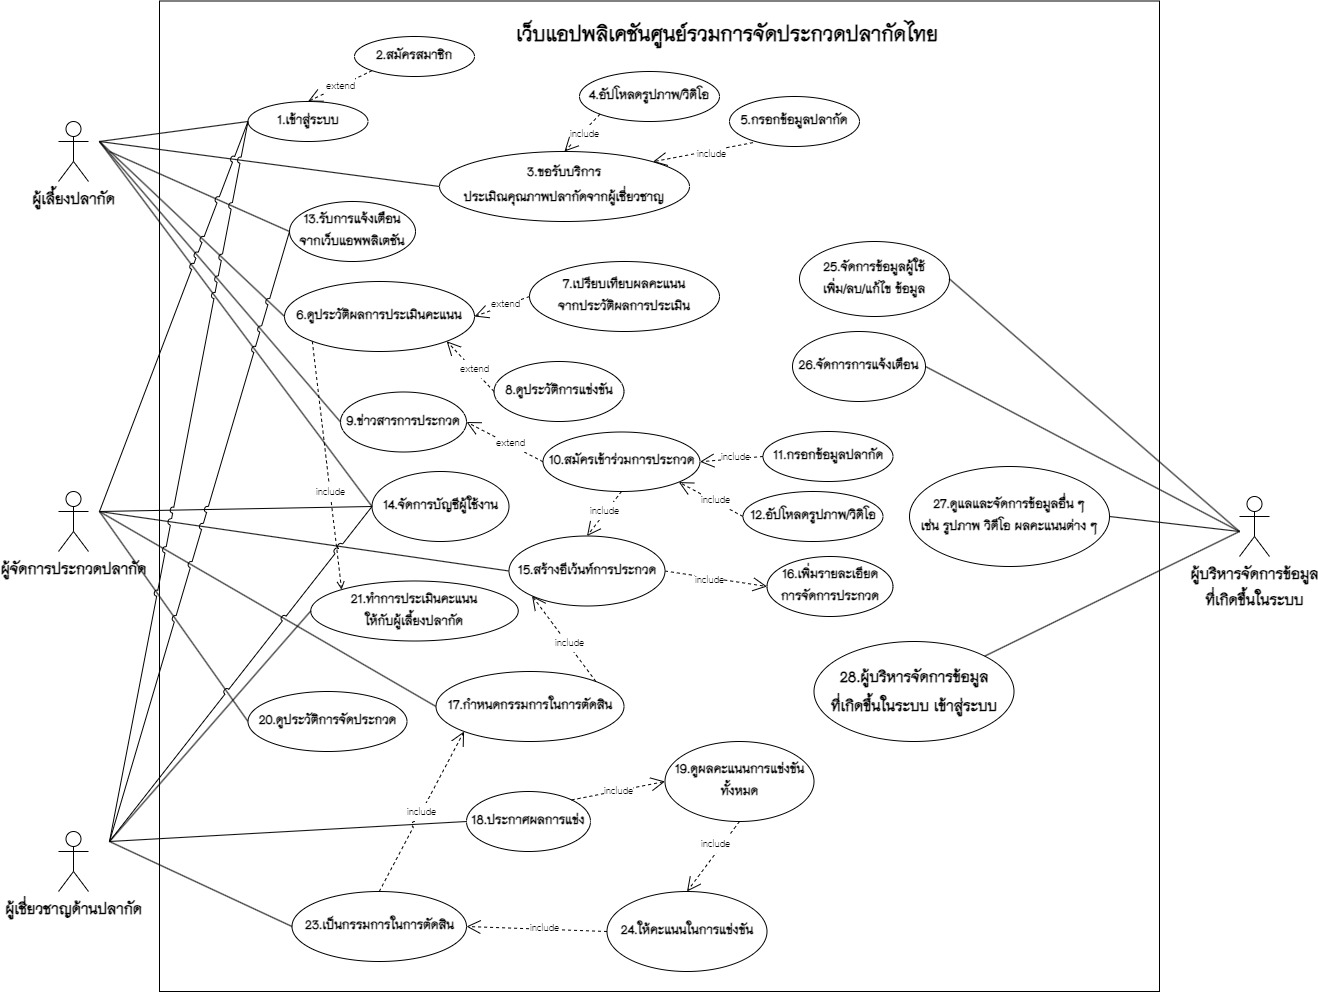
\includegraphics[width=0.8\linewidth]{Pasted image}
	\caption{Use Case ระบบเว็บแอปพลิเคชันศูนย์รวมการจัดประกวดปลากัดไทย}
\end{figure}

% ตั้งค่าให้เหมือนสเปกเดิมทุกบท
\setlength{\LoneLabelSep}{0.5em}
\settowidth{\LoneLabelWidth}{9.}
\setlength{\LoneContentCol}{\dimexpr 1.5cm + \LoneLabelWidth + \LoneLabelSep\relax}

\setlength{\LtwoLabelSep}{0.5em}
\settowidth{\LtwoLabelWidth}{9.9.}
\setlength{\ExtraAlign}{-2.8em}

% ระดับ 1: อินเดนต์ 1.5 ซม.
\setlist[enumerate,1]{%
	label=\arabic*., align=left,
	leftmargin=1.5cm, labelindent=0pt,
	labelwidth=\LoneLabelWidth, labelsep=\LoneLabelSep,
	itemsep=0pt, topsep=0.5\baselineskip
}

\begin{enumerate}
	\item Use Case: เข้าสู่ระบบ
	\item Use Case: สมัครสมาชิก
	\item Use Case: ขอรับบริการประเมินคุณภาพปลากัดจากผู้เชี่ยวชาญ
	\item Use Case: อัปโหลดรูปภาพ/วิดีโอ
	\item Use Case: กรอกข้อมูลปลากัด
	\item Use Case: ดูประวัติผลการประเมินคะแนน
	\item Use Case: เปรียบเทียบผลคะแนนจากประวัติผลการประเมิน
	\item Use Case: ดูประวัติการแข่งขัน
	\item Use Case: ข่าวสารการประกวด
	\item Use Case: สมัครเข้าร่วมการประกวด
	\item Use Case: กรอกข้อมูลปลากัด
	\item Use Case: อัปโหลดรูปภาพ/วิดีโอ
	\item Use Case: รับการแจ้งเตือนจากเว็บแอปพลิเคชัน
	\item Use Case: จัดการบัญชีผู้ใช้งาน
	\item Use Case: สร้างอีเว้นท์การประกวด
	\item Use Case: เพิ่มรายรายละเอียดการจัดการประกวด
	\item Use Case: กำหนดกรรมการในการตัดสิน
	\item Use Case: ประกาศผลการแข่งขัน
	\item Use Case: ดูผลคะแนนการแข่งขันทั้งหมด
	\item Use Case: ดูประวัติการจัดประกวด
	\item Use Case: ให้บริการประเมินคุณภาพปลากัดทำการประเมินคะแนนให้กับผู้เลี้ยงปลากัด
	\item Use Case: เป็นกรรมการในการตัดสิน
	\item Use Case: ให้คะแนนในการแข่งขัน
	\item Use Case: จัดการข้อมูลผู้ใช้ เพิ่ม/ลบ/แก้ไข ข้อมูล
	\item Use Case: จัดการการแจ้งเตือน
	\item Use Case: ดูแลและจัดการข้อมูลอื่นๆ เช่นรูปภาพ วิดีโอ ผลคะแนนต่างๆ
	\item Use Case: ผู้บริหารจัดการข้อมูลที่เกิดขึ้นในระบบ เข้าสู่ระบบ
\end{enumerate}

\vspace{\baselineskip}

% ================== Use Case: Login ==================
\begin{table}[h]
	\caption{Use Case สำหรับการเข้าสู่ระบบ}
	{\tablefont
		\setlength{\tabcolsep}{6pt}%
		\begin{tabularx}{\linewidth}{@{} >{\justifying\arraybackslash}X >{\raggedleft\arraybackslash}p{4.2cm} @{}}
			\Xhline{1.5pt}
			\textbf{Use Case Title:}\enspace เข้าสู่ระบบ & \UseCaseID[uc:login] \\
			\Xhline{0.5pt}
			\textbf{Primary Actor:}\enspace ผู้เลี้ยงปลากัด, ผู้จัดการประกวด, ผู้เชี่ยวชาญด้านปลากัด, ผู้บริหารจัดการข้อมูลที่เกิดขึ้นในระบบ & \\
			\Xhline{0.5pt}
			\textbf{Stakeholder Actor:}\enspace - & \\
			\Xhline{0.5pt}
			\textbf{Main Flow:}\enspace สามารถกรอก username และ password เข้าสู่ระบบใช้งานได้เลยกรณีมีบัญชีผู้ใช้งานอยู่แล้ว & \\
			\Xhline{0.5pt}
			\textbf{Exception Flow ที่ 1:}\enspace กรณีที่ผู้ใช้งานยังไม่มีบัญชีเข้าใช้งาน ระบบจะแจ้งเตือนให้ผู้ใช้สมัครสมาชิกก่อนเข้าใช้งานเว็บแอพพลิเคชัน & \\
			\Xhline{1.5pt}
		\end{tabularx}
	}
\end{table}
% =====================================================



\clearpage